\chapter{\samptr{} Additional Materials}\label{sec:samptr-additional-mat}

This chapter covers the motivation for \samptr{}'s design choices as well as additional experiments with different types of graph neural networks.

Based on the discussion in \Cref{sec:ccclr-additional-mat}, there are three main issues with \ccclr{} that we have to address:
\begin{enumerate}
    \item There is no constraint on the amount of elements that can be placed within a cluster
    \item It is computationally heavy to compute new clusters in each training step 
    \item Partial compatibility with gradient-based learning hinders the network's learning ability (previous knowledge about re-ranking and clustering does not carry over).
\end{enumerate}

These problems with \ccclr{} formed the basis for certain design choices with respect to \samptr{}. In order to tackle problem (1), we do away with the clustering step and instead rely on self-attention based message passing to discover and refine features that belong to the same overarching class. In \ccclr{}, the clustering step was used to find similar data points in a batch. The same can be achieved by means of a self-attention message passing (SAMP) layer, because the SAMP layer can weigh the importance of each sample in its neighbourhood, it can also discover samples that are similar to each other.

For problem (2), we no longer need to use a heavy clustering and re-ranking steps. Both of these tasks can be handled by the self-attention message passing layer. Not only is it able to detect similar images in a batch (replaces clustering), it can also refine their features to bring them closer (replaces re-ranking).

For problem (3), as described in \cref{chap:gnn} graph neural networks are fully compatible with gradient based learning and optimisation. 


\section{Why SAMP?}\label{sec:why-samp}

\Cref{tab:gnn-types} shows the performance of three different types of GNNs. Before arriving on SAMP, we also tested the dynamic edge convolutions \parencite{wang2019dynamic} and LatentGNN \parencite{zhang2019latentgnn} layers.

\begin{table}[ht]
    \centering
    \begin{tabularx}{290pt}{Y Y Y}
    \toprule
        \textbf{Backbone} & \textbf{GNN Type} & \textbf{Accuracy} \\ 
        \midrule
        Conv4 & EdgeConv \citeyearpar{wang2019dynamic} & 57.76 $\pm$ 0.81 \\
        Conv4 & LatentGNN \citeyearpar{zhang2019latentgnn} & \underline{61.07} $\pm$ 0.66 \\
        Conv4 & SAMP  & \textbf{64.67} $\pm$ 2.65 \\
        \bottomrule
    \end{tabularx}
    \caption{Comparision between three types of GNN layers. Accuracy ($\%$ $\pm$ std.) values are for (\nwks{5}{5}) \miniImagenet{} classification tasks.}
    \label{tab:gnn-types}
\end{table}

We chose the EdgeConv layer because it has the ability to dynamically update the graph at every step. EdgeConv was originally developed to be used in processing 3D point cloud data, where it was meant to grasp the 3D structure of and relationships between the points of a scanned item.
We expected it to perform well with image feature vectors; however, due to the data changing too rapidly between training steps, it proved challenging for the EdgeConv layer to learn the similarities and relationships between images.

The next layer that we tested was the LatentGNN layer \parencite{zhang2019latentgnn}. It was developed for the express purpose of modelling non-local contextual relations between visual feature maps. The key idea is to introduce a latent space to reduce the complexity of the graph, which allows the use of a low-rank representation for the graph affinity matrix. \textcite{zhang2019latentgnn} insert this layer at intermediate points in a ResNet-$50$ and ResNet-$101$ \parencite{He2015}. The layer projects square feature maps to latent space as feature vectors and then applies message passing steps to refine the feature vectors and finally converts them back to square feature maps for further processing by convolution blocks.
Although this layer showed promising results, it requires a LatentGNN layer to be placed between convolutional layers, making a simple Conv$4$ unreasonably complex. However, the results were close enough to \ccclr{} and other competitors that it made natural sense to explore this direction further.

Ultimately, we arrive at a variant of the graph attention (GAT) layer \parencite{velic018graph} that we have coined as SAMP. SAMP has been formulated by \parencite{brody2021attentive,seidenschwarz2021learning}, among others. To the best of our knowledge, no one seems to have used it in the unsupervised few-shot learning context. It is simpler to use than LatentGNN and with minimal tuning the performance was within the margin of error of \ccclr{}.

\section{SAMP in Action}\label{sec:samp-in-action}

In \cref{fig:samp-training-emb-plots} the plot on the right shows image augmentations tightly grouped around the source image. From this we can infer that the SAMP layer is able to recognise similar images and refine their features so that they are closer in the representation space.
\begin{figure}[h]
     \centering
     \begin{subfigure}[b]{0.4\textwidth}
         \centering
         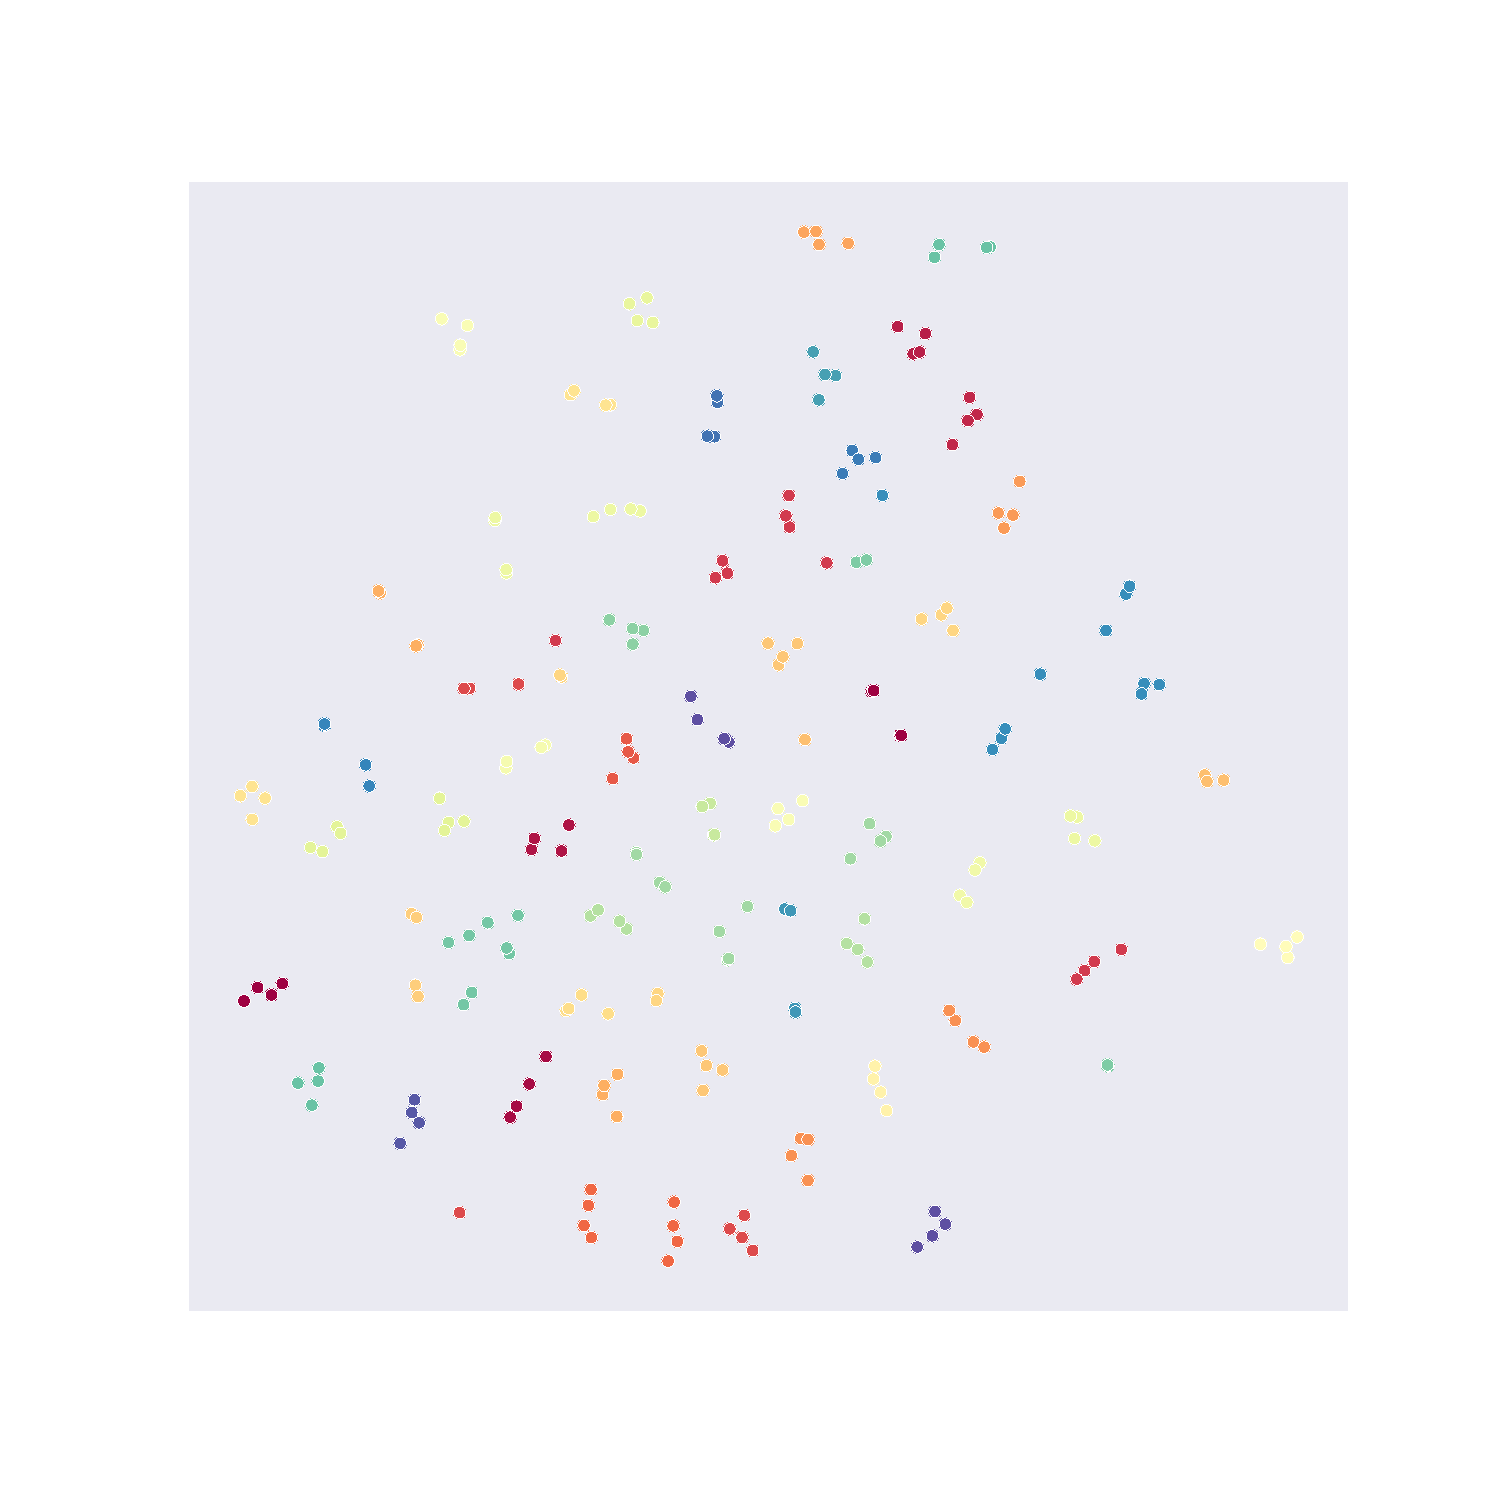
\includegraphics[width=\textwidth,trim=2.55cm 3cm 2.6cm 2.6cm, clip]{chapters/assets/samptr_extra/cnn_emb.pdf}
     \end{subfigure}
     \hspace{1cm}
     \begin{subfigure}[b]{0.4\textwidth}
         \centering
         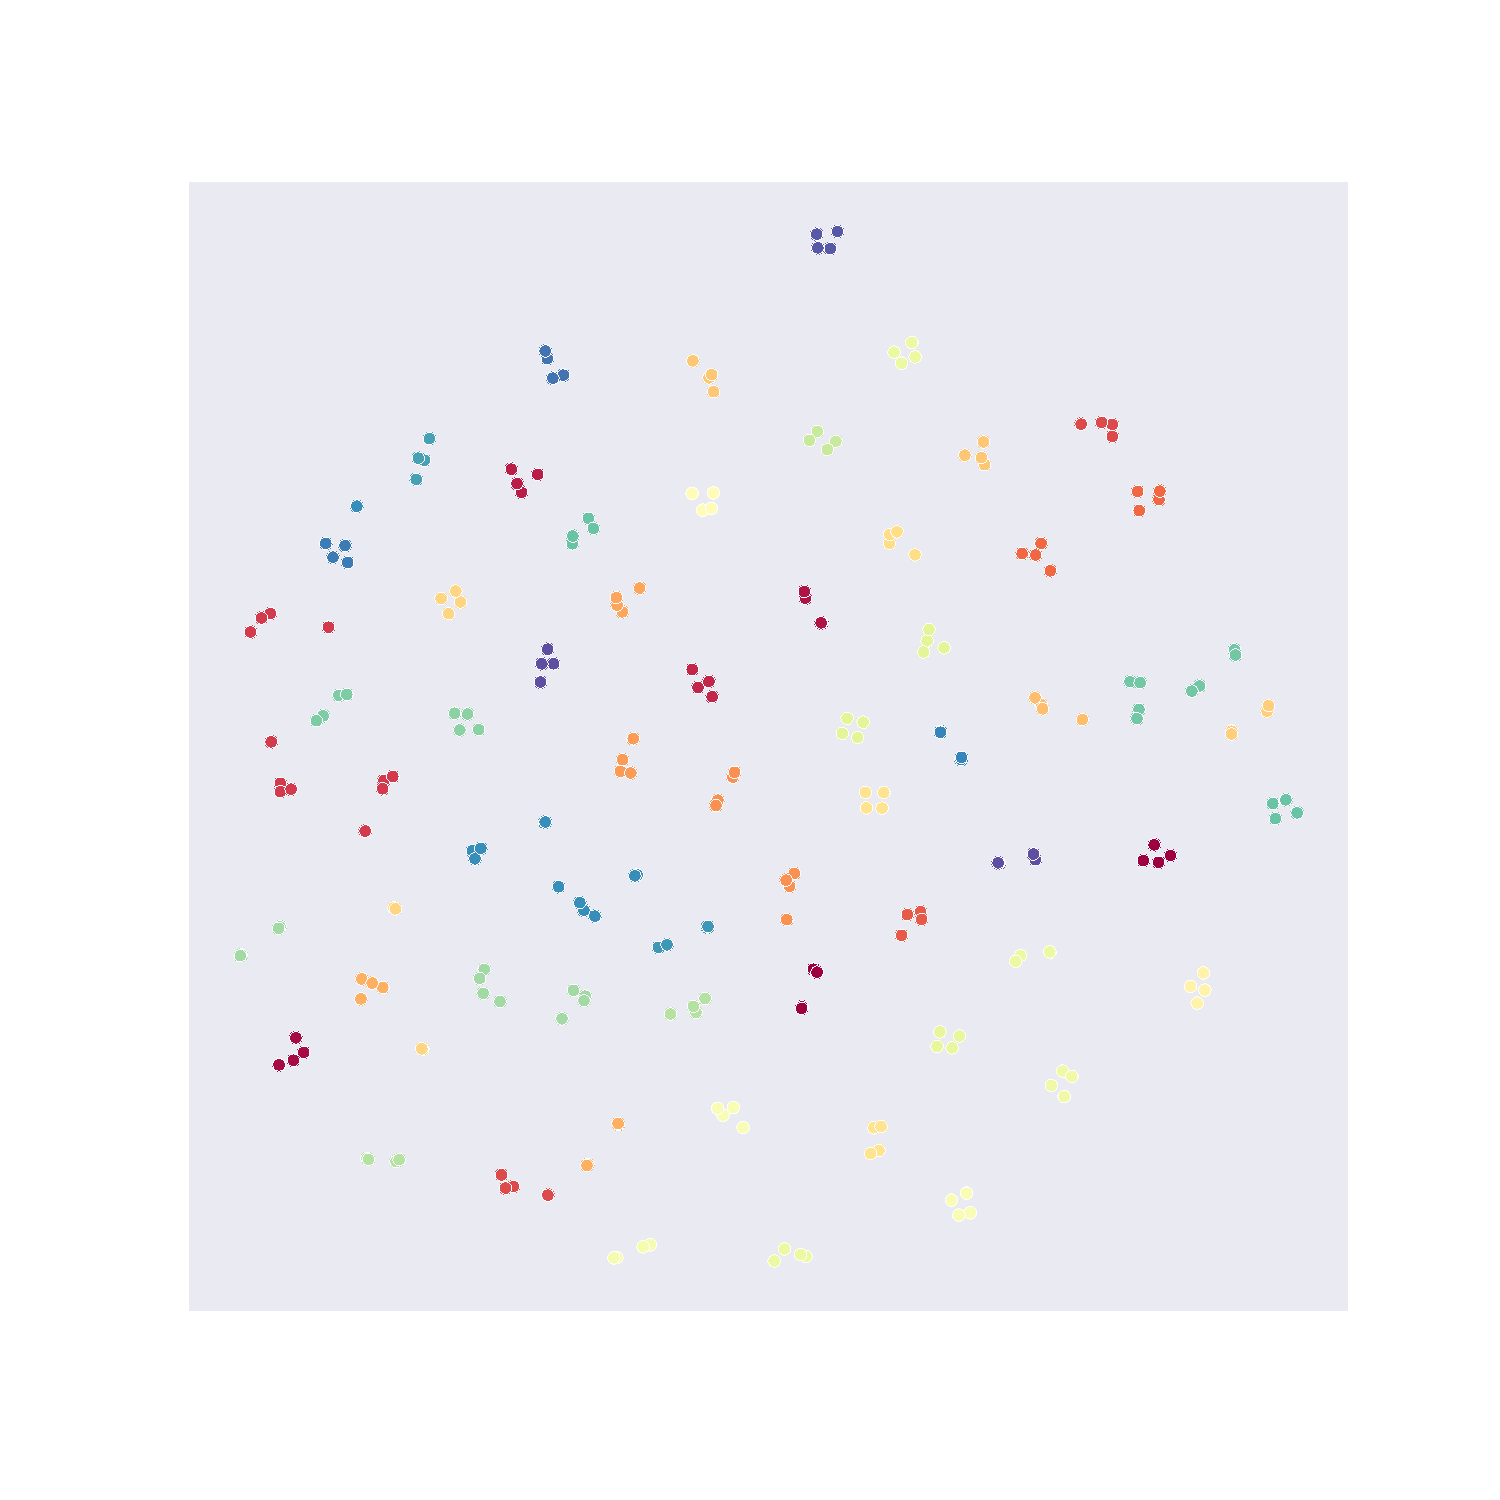
\includegraphics[width=\textwidth, trim=2.55cm 3cm 2.6cm 2.6cm, clip]{chapters/assets/samptr_extra/gnn_emb.pdf}
     \end{subfigure}
     \caption{ Each point is an image representation that has three neighbours which are its augmentations. The UMAP plot on the left shows features generated by the Conv$4$ backbone, the points are clearly more spread out. The flattened output of the Conv$4$ backbone are used as input to the SAMP layer. The UMAP plot on the right generated by using the SAMP layer outputs.
     }
     \label{fig:samp-training-emb-plots}
\end{figure}

Similar to \cref{fig:samp-training-emb-plots}, \cref{fig:samp-val-emb-plots} shows the embeddings of a support and query set in a (\nwks{2}{5}) task. We can see that the CNN features on the left aren't as separable, several \textcolor{orange}{orange} dots are in the are of the \textcolor{green}{green cluster}. However, when the CNN features are passed through a \texttt{SAMP} layer we can see that clusters form that are almost perfectly separable, indicating that the \texttt{SAMP} layer is working by looking beyond single instances and has learnt to refine features as required.

\begin{figure}[h]
     \centering
     \begin{subfigure}[b]{0.4\textwidth}
         \centering
         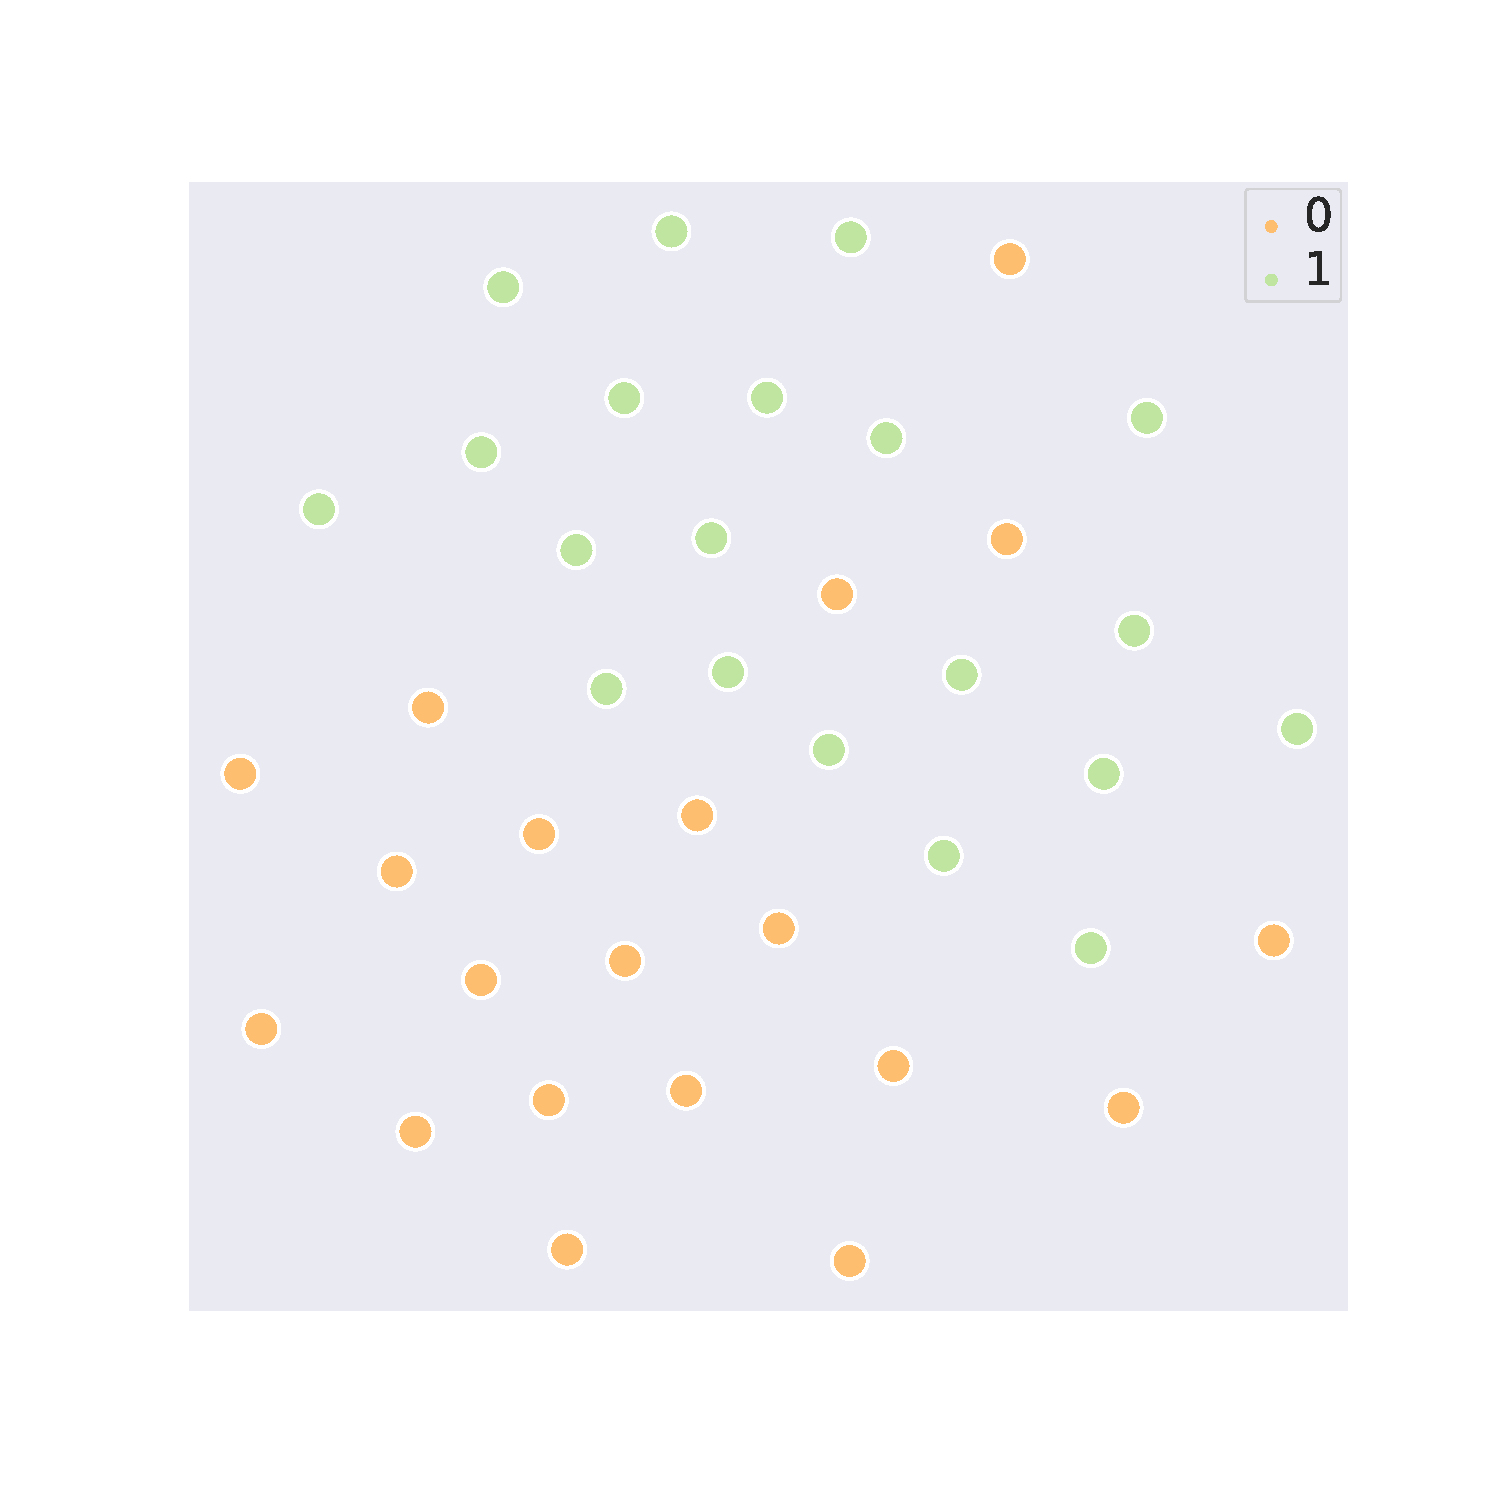
\includegraphics[width=\textwidth,trim=2.55cm 3cm 2.6cm 2.6cm, clip]{chapters/assets/samptr_extra/cnn_val_emb.pdf}
     \end{subfigure}
     \hspace{1cm}
     \begin{subfigure}[b]{0.4\textwidth}
         \centering
         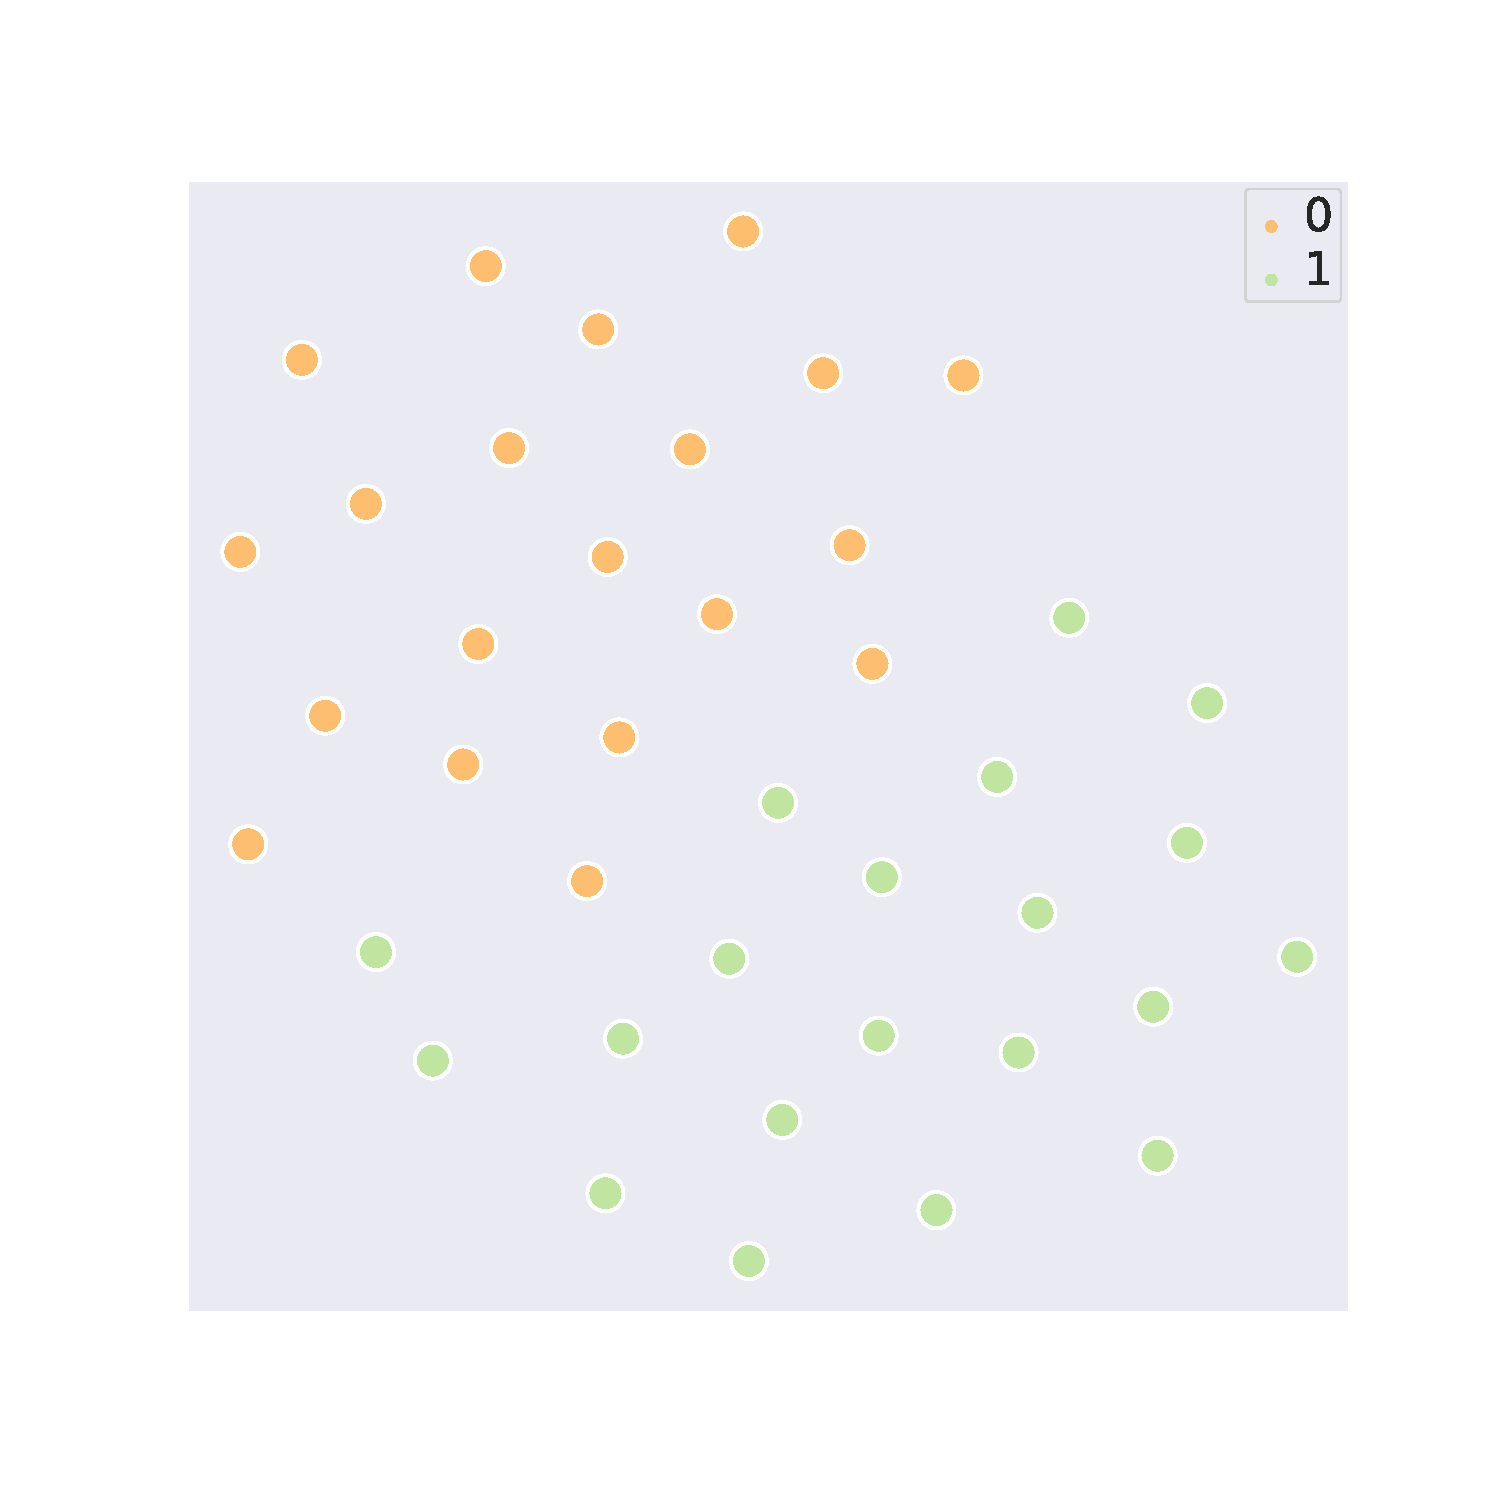
\includegraphics[width=\textwidth, trim=2.55cm 3cm 2.6cm 2.6cm, clip]{chapters/assets/samptr_extra/gnn_val_emb.pdf}
     \end{subfigure}
     \caption{The figure on the left shows the CNN features of a support and query set from (\nwks{2}{5}) task drawn from the \miniImagenet{} validation set. The figure on the right shows the SAMP refined features where we can see two clearly separated clusters of points whereas on the right there are a few stray \textcolor{orange}{orange} points.}
     \label{fig:samp-val-emb-plots}
\end{figure}